\subsubsection{Orbit Test}
\label{sec.test.testorbit}

\begin{figure}
\begin{center}
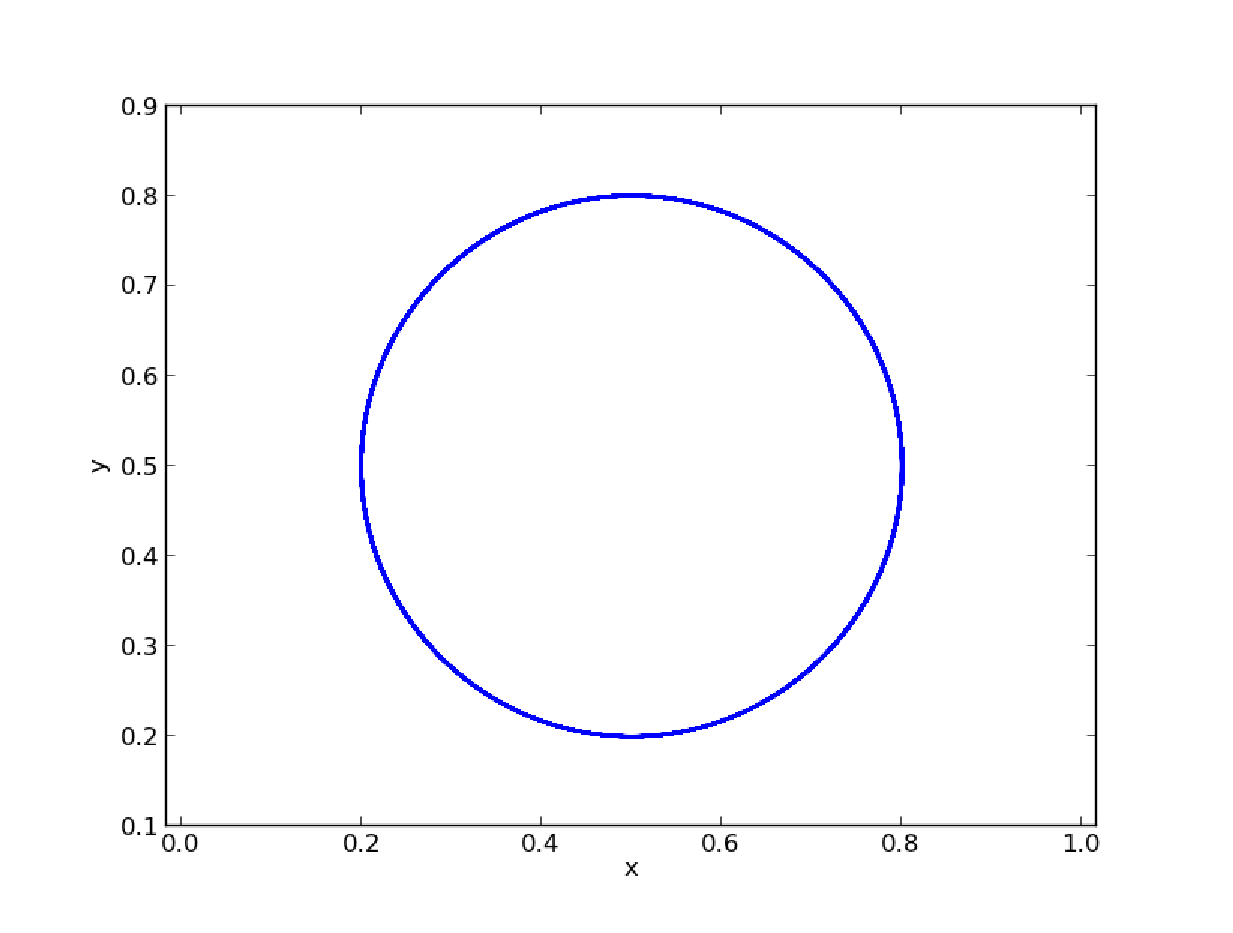
\includegraphics[width=0.45\textwidth]{figures/TestOrbit_xy.eps}
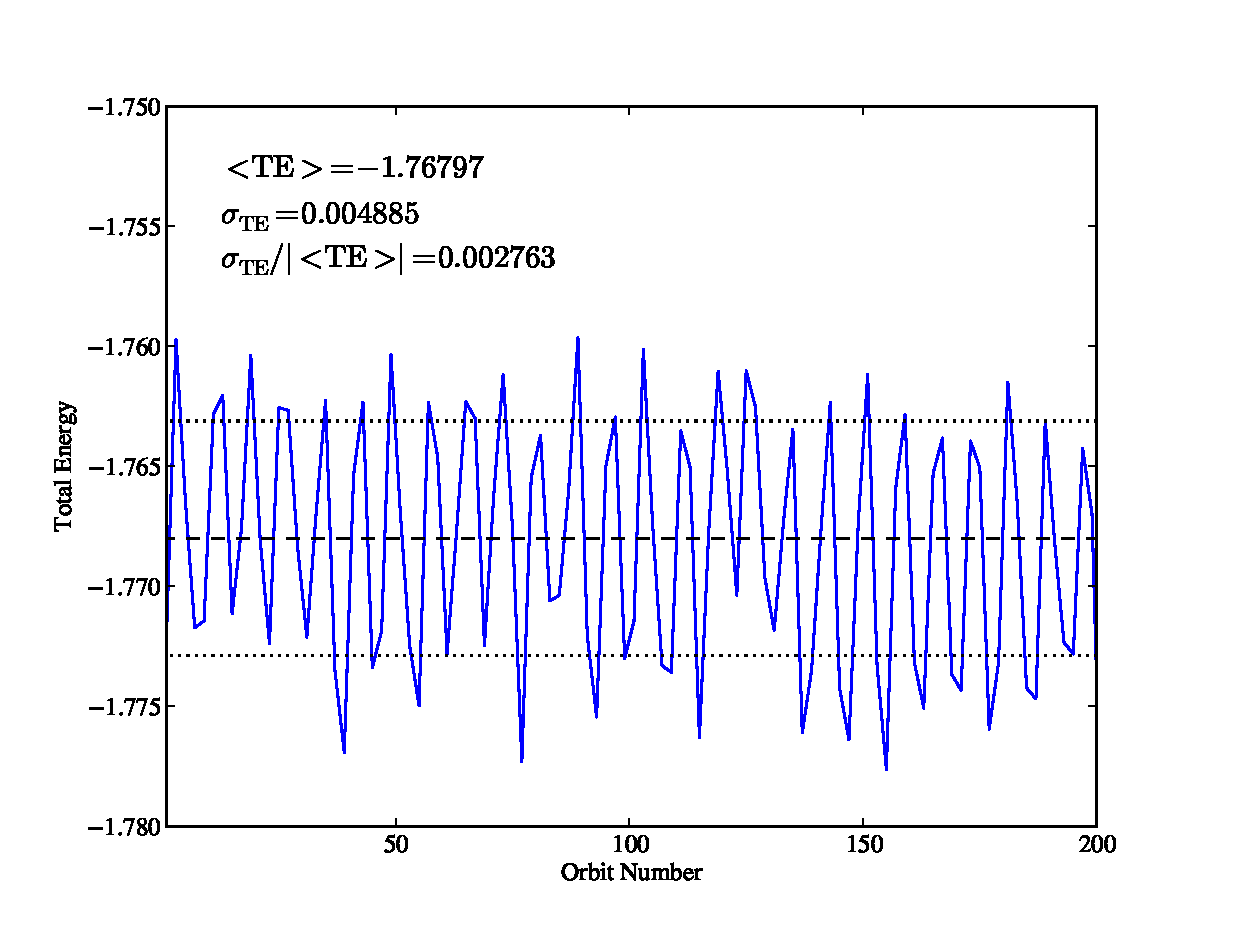
\includegraphics[width=0.45\textwidth]{figures/TestOrbit_TotalEnergy.eps}
\caption{Test particle behavior in the Orbit problem, which is used to
test the gravity solver and particle integration.  An effectively
massless test particle is set in circular orbit around a massive
central particle, with the gravitational potential calculated on a 3D,
$32^3$ grid, and evolved forward in time for 200 orbits.  Left panel:
path of the test particle in the orbital plane plotted for the
duration of the simulation, with a zoomed box showing a small portion
of the orbit to highlight deviations from perfect circularity.  Right panel: total specific energy
(kinetic plus potential) for the test particle for the duration of the
simulation.  The particle's mean energy (integrated over the length of
the simulation) is represented by a horizontal dashed line, and +/-
one standard deviation by horizontal dotted lines.  All quantities are
in arbitrary units.}
\label{fig.orbittest}
\end{center}
\end{figure}

The ``orbit test'' simulates the orbit of an effectively massless
particle around a massive primary particle and is used to test the
accuracy of both the gravity solver and particle integration.  In this
problem (shown in Figure~\ref{fig.orbittest}), a 3D box with unit size
and a $32^3$ grid is created, and a particle with mass 1 is placed at
the center of the box (both box length and particle mass are in
arbitrary units).  A second ``test'' particle, with mass of $10^{-6}$,
is placed at a distance of 0.3 L$_{box}$ from the primary particle in
the x-y plane (at $z=0.5$~L$_{box}$).  Both particles are given
velocities such that they will orbit their common center of mass in
the x-y plane.  The simulation is run for 200 orbits, writing
out a dataset 
approximately once per orbit (with the particle positions being
written out several hundred times per orbit).

The left panel of Figure~\ref{fig.orbittest} shows the path of the
test particle in the x-y plane (at z=$0.5$), plotted over the duration
of the simulation.  The test particle
maintains a path that has effectively unnoticeable deviation from
circularity, and with no discernable drift in either net radius or
orbit center over time.  The right panel displays the total specific
energy of the test particle (defined as $\frac{1}{2} {\bf v}^2 +
\phi$, where $\phi$ is the gravitational potential at the position of
the test particle) as a function of time, plotted once per orbit.  The
mean total specific energy is $-1.76797$ in arbitrary units, with a
standard deviation of $0.004885$ ($0.276\%$ of the mean value), and
with a maximum deviation from the mean of $0.546\%$ of the mean value.
Given that the potential is calculated on $32^3$ cells, the two
particles are separated by between 10 and 14 cells depending on their
relative positioning in the grid, and the particles are integrated
using a second-order leapfrog method, this level of accuracy is
expected and acceptable.
